\section{How to beat the Go world champion - AlphaGo}
\begin{frame}{}
    \LARGE How to Beat the Go World Champion: \textbf{AlphaGo}
\end{frame}

\begin{frame}{How to Beat the Go World Champion - AlphaGo}
\begin{figure}
\centering
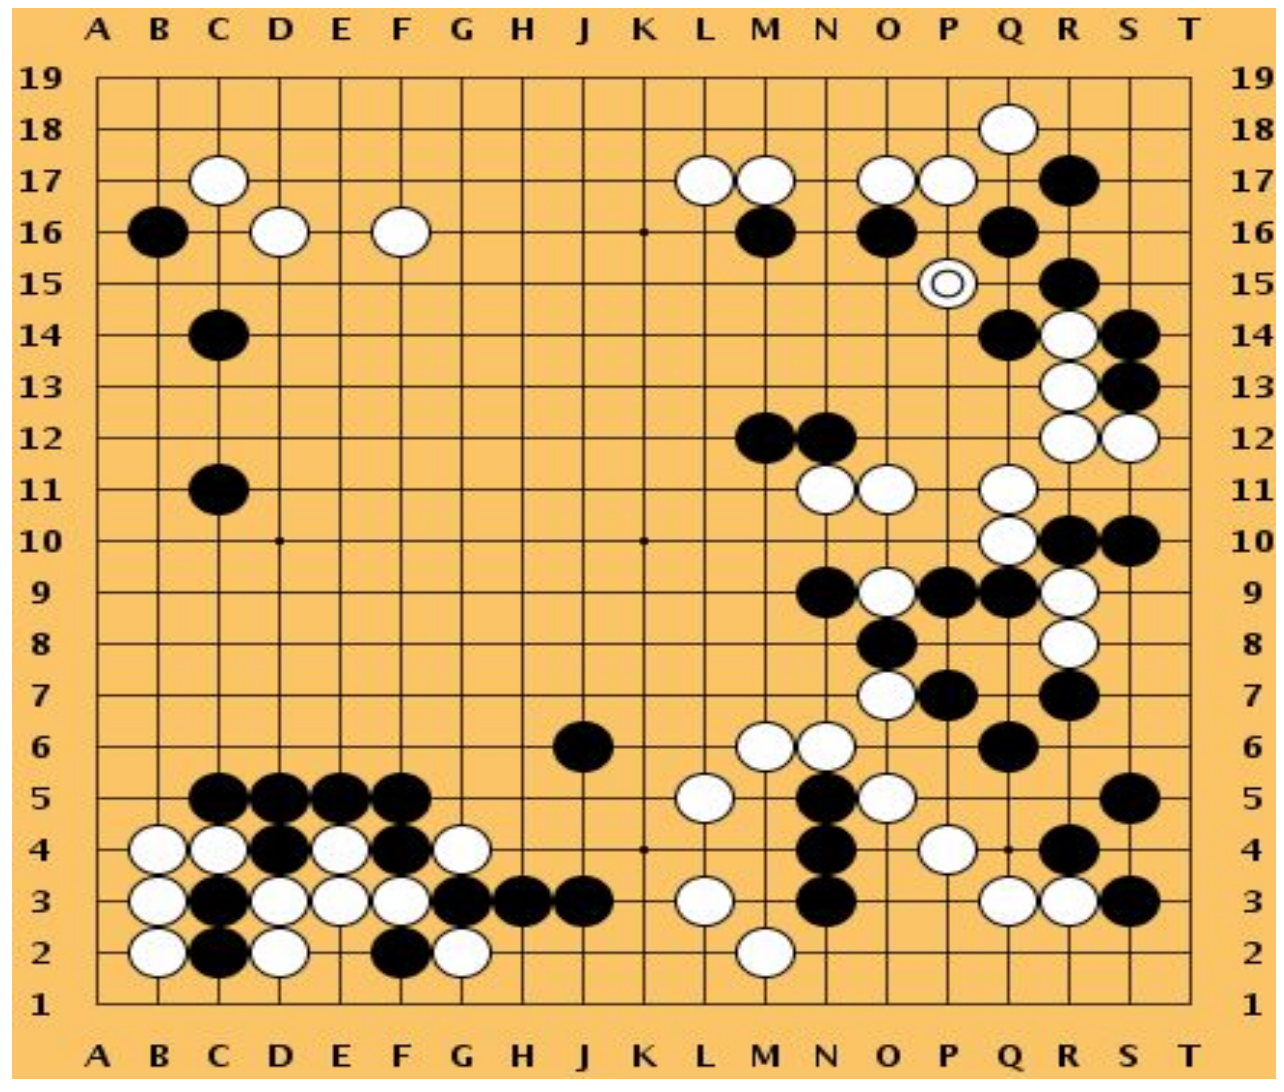
\includegraphics[width=0.9\textwidth,height=0.6\textheight,keepaspectratio]{images/policygrad+reinforce+actor/alphago.png}
\end{figure}

\begin{itemize}
    \item Combination of supervised learning and reinforcement learning
    \item Integration of traditional methods (Monte Carlo Tree Search) with modern approaches (deep reinforcement learning)
\end{itemize}
\footnotetext{[Silver et al., Nature 2016]}
\end{frame}

\begin{frame}{How to Beat the Go World Champion - AlphaGo}
\begin{itemize}
    \setlength{\itemsep}{1em}
    \large
    \item Featurize the board (stone color, move legality, biases, etc.)
    \item Initialize the policy network with supervised training on professional Go games, then continue training using policy gradients (self-play from random previous iterations, with +1/-1 reward for winning/losing)
    \item Learn a value network (critic) to estimate the value of board positions
    \item Finally, combine the policy and value networks within a Monte Carlo Tree Search algorithm to select actions via lookahead search
\end{itemize}
\footnotetext{[Silver et al., Nature 2016]}
\end{frame}
